This section implements heuristics for generating test inputs.  I'll use the
HTTP tester as an example to show how to make requests more interesting by
parameterizing them over the model state (\autoref{sec:heuristic-state}) and the
trace (\autoref{sec:heuristic-trace}).

\subsection{State-based heuristics}
\label{sec:heuristic-state}
The model state may instruct the test generator to produce more interesting test
inputs.  For example, consider the \ilc{random_path} generator in
\autoref{line:random-path} of \autoref{fig:naive-generator}.  One way to improve
it is to generate more paths that have corresponding resources on the server:
\begin{coq}
  Definition gen_path (state: list (path * resource)) : IO path :=
    let paths: list path := map fst state in
    freq [(90, oneof paths);
          (10, random_path)].
\end{coq}

Here I modify the server model's state type \ilc{sigma} from \ilc{(path ->
  resource)} in \autoref{fig:if-match-server} into \ilc{(list (path *
  resource))}, which allows the generator to access the list of all \ilc{paths}
  in the server state.  The generator chooses from these existing paths in 90\%
  of the cases, as assigned by the \ilc{freq} combinator.  The remaining 10\%
  are still generated randomly, to discover how the SUT handles nonexistent
  paths.

For the \ilc{gen_packet} generator in \autoref{fig:naive-generator}, replacing
its \ilc{random_path} with the improved \ilc{gen_path} would generate more
interesting request targets.  This requires the \ilc{gen_packet} to carry the
server state to instantiate \ilc{gen_path}.

As shown in \autoref{fig:backtrack}, the \ilc{GenPacket} generator is triggered
when the tester wants to observe a packet from itself to the SUT.
\autoref{fig:symbolic-observer} then shows that such \ilc{FromObserver} expectation
happens when the symbolic model \ilc{Send}s a packet.  Such a \ilc{Send} event
only happens when the server wants to receive a packet in
\autoref{fig:net-compose}.  The \ilc{Recv} events are triggered by the server
model in \autoref{fig:if-match-server}, which iterates over the server state
\ilc{sigma}.

Therefore, I extend the symbolic server model's \ilc{Recv} event type on
Page~\pageref{def:symbolic-qae} to include the server state:
\begin{coq}
  Variant qaE: Type -> Type :=
    Recv : sigma      -> qaE packet
  | Send : packet -> qaE unit.
\end{coq}

Now when the server wants to receive a request, it triggers \ilc{(Recv state)},
where \ilc{(state: sigma)} contains the server's paths and resources at that
point.  The \ilc{state} argument is then carried to the generator, by adding
parameters to the event types along the interpretation:
\begin{coq}
  Variant netE: Type -> Type :=
    Emit  : packet -> netE unit
  | Absorb: sigma      -> netE packet.

  Variant observeE : Type -> Type :=
    FromObserver   : sigma -> observeE concrete_packet
  | ToObserver     : observeE concrete_packet.

  Variant genE: Type -> Type :=
    GenPacket : sigma -> genE concrete_packet
  | GenBool   : genE bool.

  Definition gen_packet: sigma -> IO concrete_packet.
\end{coq}

\begin{figure}
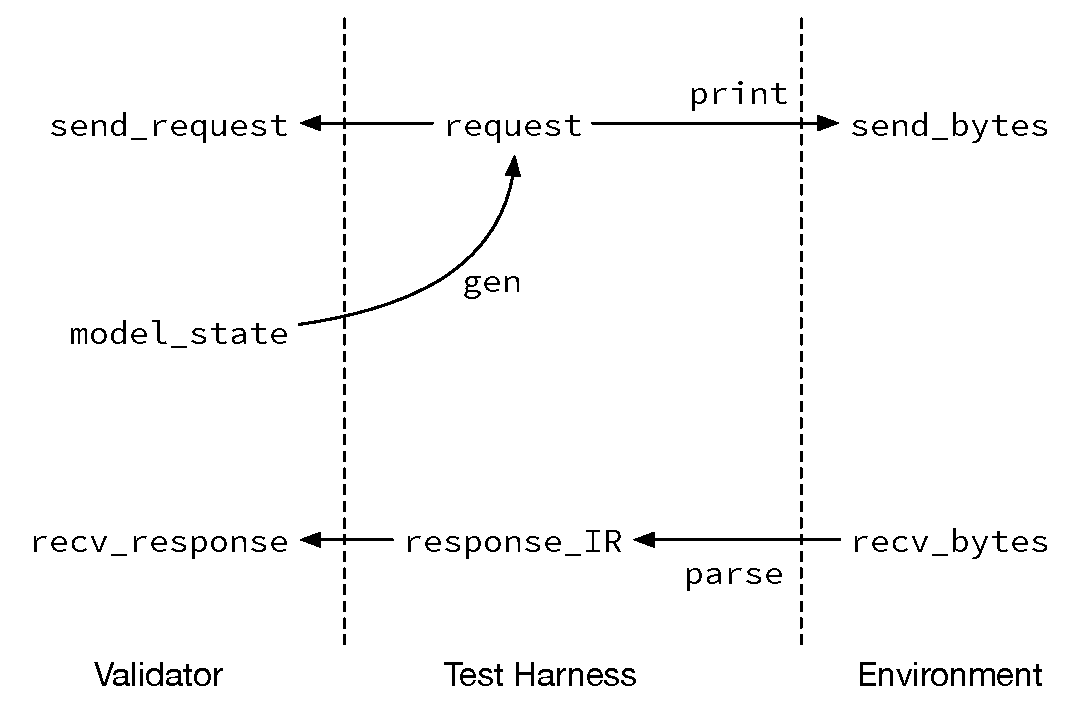
\includegraphics[width=.6\linewidth]{figures/stategen}
\caption{State-based heuristics.}
\label{fig:stategen}
\end{figure}

As a result, when instantiating the \ilc{(GenPacket state)} event in
\autoref{fig:execute}, we can feed the \ilc{gen_packet} function with argument
\ilc{state}, so that \ilc{gen_path} can generate interesting paths based on the
server state.  \autoref{fig:stategen} illustrates this state-based heuristics.
It refines the test harness box in \autoref{fig:overview}, and will be extended
with trace-based heuristics in the next subsection.

\subsection{Trace-based heuristics}
\label{sec:heuristic-trace}

When the SUT makes internal choices, e.g., generating ETags, the
specification represents them as symbolic variables.  These variables' concrete
value are not stored in the specification state, but may be observed during
execution.  For example, when an HTTP server responds to a GET request, it might
include the resource's ETag as shown in \autoref{sec:internal-nondeterminism}.

To improve the generator in \autoref{fig:naive-generator}, we can generate
interesting ETags based on the trace produced during execution.  The trace is a
list of packets sent and received by the tester, and the packets' payloads may
include responses that have an ETag field.  The \ilc{gen_etag} function
emphasizes ETags that were observed in the trace, which are more likely to match
those generated by the SUT:
\begin{coq}
  Definition gen_etag (trace: list concrete_packet) : IO string :=
    let etags: list string := tags_of trace in
    freq [(90, oneof etags);
          (10, random_etag)].
\end{coq}

To utilize this improved generator for ETags, the tester needs to record the
trace of packets sent and received.  This is done by modifying the \ilc{execute}
function in \autoref{fig:execute}, adding an accumulator as the recursion parameter:
\begin{coq}
  Fixpoint execute (fuel: nat) (trace: list concrete_packet)
                   (m: itree tE void) : IO bool :=
    match fuel with
    | S fuel' =>
      match m with
      | Impure e k =>
        match e with
        | (ClientSend q|) => client_send q;;
                             execute fuel' (trace ++ [q]) (k tt)
        | (ClientRecv|)   => oa <- client_recv;;                             
                             let trace' := match oa with
                                           | Some a => trace ++ [a]
                                           | None   => trace
                                           end in
                             execute fuel' trace' (k oa)
        | (|GenPacket state|) => pkt <- gen_packet state trace;;
                                 execute fuel' trace (k pkt)
        ... (* similar to %\autoref{fig:execute}% *)
\end{coq}

When the tester sends or receives a packet, the packet is appended to the
runtime \ilc{trace}.  Then the \ilc{gen_packet} generator can take the trace
accumulated so far and feed it to the ETag generator:
\begin{coq}
  Definition gen_packet (state: sigma) (trace: list concrete_packet) :=
    target <- gen_path state;;
    etag   <- gen_etag trace;;
    ... (* same as %\autoref{fig:naive-generator}% *)
\end{coq}

\begin{figure}
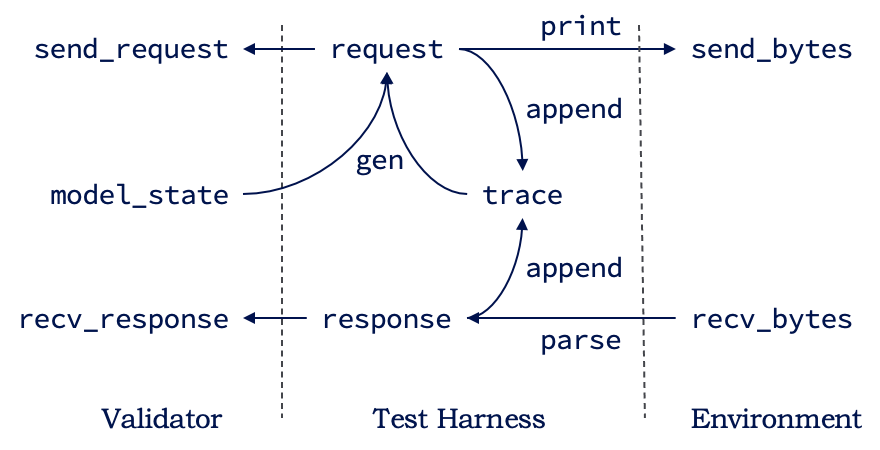
\includegraphics[width=.7\linewidth]{figures/gen}
\caption{Combining state-based and trace-based heuristics.}
\label{fig:gen}
\end{figure}

Now we can generate interesting test inputs by combining state-based and
trace-based heuristics, as shown in \autoref{fig:gen}.  In the next section,
I'll further extend this framework and shrink the test inputs while keeping them
interesting, addressing inter-execution nondeterminism.
